%%%%%
%%%%% Supporting material for Sandwich paper.
%%%%% Compile with pdflatex as figures are not eps.
%%%%%
\documentclass[12pt,twoside]{article}
\usepackage{graphicx}

\setlength{\hoffset}{-1in}
\setlength{\voffset}{-1in}

\setlength{\topmargin}{2cm}
\setlength{\evensidemargin}{3.1cm}
\setlength{\oddsidemargin}{3.1cm}

\setlength{\textwidth}{14.8cm}
\setlength{\textheight}{23cm}

\setlength{\parindent}{0pt}
\setlength{\parskip}{\medskipamount}
\pagestyle{empty}


\begin{document}


{\bf Supporting Online Material: Sandwich Title}

Here, the details of the simulation method, protocol, and parameters are
set out. The matching of simulation units to physical units is also
discussed.

{\bf 1. Thermodynamics}

The thermodynamics of the cholesteric liquid crystal can be described
by means of a  Landau-de Gennes free energy functional $\cal F$,
whose density is written as $f$:
\begin{eqnarray}
{\cal F}[{\bf Q}]&=&\int d^3{\bf r} f({\bf Q}({\bf r})).
\end{eqnarray}
This free energy density $f = f({\bf Q})$ may be expanded in powers of the
order parameter ${\bf Q}$ and its gradients; ${\bf Q}$ is a traceless 
and symmetric tensor which we will denote from now on in subscript
notation as $Q_{\alpha\beta}$.
The largest eigenvalue $q$ and corresponding eigenvector $n_\alpha$
of $Q_{\alpha\beta}$ describe the local strength and major orientation axis
of molecular order.
The theory based on the tensor $Q_{\alpha\beta}$, rather than a theory based
solely
on the director field $n_\alpha ({\bf r})$, allows treatment of disclinations
(defect lines) in whose cores $n_\alpha$ is undefined.

Explicitly, the free energy density is:
\begin{eqnarray}
f(Q_{\alpha\beta}) &=& {\textstyle \frac{1}{2}} A_0
 \left(1- {\textstyle \frac{1}{3}}\gamma \right)Q^2_{\alpha \beta}
-{\textstyle \frac{1}{3}}A_0\gamma Q_{\alpha \beta} Q_{\beta \gamma}Q_{\gamma \alpha} 
+ {\textstyle \frac{1}{4}} A_0\gamma (Q^2_{\alpha \beta})^2  \nonumber\\
&+& {\textstyle \frac{1}{2}} K(\varepsilon_{\alpha \gamma \delta}
\partial_\gamma Q_{\delta \beta} + 2 q_0 Q_{\alpha \beta})^2
+ {\textstyle \frac{1}{2}} K (\partial_\beta Q_{\alpha \beta})^2
\label{free}
\end{eqnarray}
Here, repeated indices are summed over, while terms of the form
$Q^2_{\alpha\beta}$ should be expanded to read $Q_{\alpha\beta}Q_{\alpha\beta}$;
$\varepsilon_{\alpha\gamma\delta}$ is the permutation tensor.
The first three terms are a bulk free energy density whose overall scale
is set by $A_0$ (discussed further below); $\gamma$ is a control parameter
related to a reduced temperature. Varying the latter in the absence of
chiral terms ($q_0=0$) gives an isotropic-nematic transition at
$\gamma = 2.7$ with a mean-field spinodal instability at $\gamma = 3$.

The remaining terms of the free energy density in Eq.~\ref{free} describe
distortions of
the order parameter field. It is conventional \cite{blue1,deGennes} to
assume that splay, bend and twist deformations of the director are equally
costly, that is, there is a single elastic constant $K$. The parameter $q_0$
is related to the helical pitch length $p$ via $q_0=2\pi/p$,
describing one full turn of the director in the cholesteric phase.

There are two dimensionless numbers, which are commonly referred to as
$\kappa$, the chirality, and  $\tau$, the reduced temperature
\cite{blue1}.  In terms of the parameters in the free energy density,
these are:
\begin{eqnarray}\label{cntrl-param} 
\tau&=&\frac{27(1-\gamma/3)}{\gamma}\label{tau}\\
\kappa&=&\sqrt{\frac{108\ K\, q_0^2}{A_0\, \gamma}}\label{kappa}.
\end{eqnarray}
If the free energy density Eq.~\ref{free} is made dimensionless, $\tau$
appears as prefactor of the term  quadratic in $Q_{\alpha\beta}$,
whereas $\kappa$
quantifies the ratio between bulk and  gradient free energy terms. The
chirality and reduced temperature may be used to characterise an equilibrium
phase diagram of the blue phases in bulk cholesteric liquid crystals
\cite{blue1,oliver1}.
In this work, the chirality and reduced temperature are always set to lie
within the blue phase I region of the equilibrium phase diagram.

In addition to the fluid free density density $f(Q_{\alpha\beta})$, a surface
free energy density is also present to represent the energetic cost of
anchoring at a solid surface. If the preferred order parameter tensor
at the solid surface is $Q^0_{\alpha\beta}$, then the surface free energy
density (per unit area) is
\begin{equation}
f_s(Q_{\alpha\beta}, Q^0_{\alpha\beta})
= {\textstyle \frac{1}{2}}W(Q_{\alpha\beta} - Q^0_{\alpha\beta})^2,
\end{equation}
where $W$ is a constant determining the strength of the anchoring.
The determination of $Q^0_{\alpha\beta}$ for normal and planar anchoring is
discussed below. For a colloid of radius $a$, the strength of the surface
anchoring compared which the bulk fluid elastic constant may be quantified
by the dimensionless parameter $Wa/K$. For small values of this parameter,
the presence of a colloid surface should have little impact on the local
fluid LC ordering.

% NO REDSHIFT

{\bf 2. Dynamics}

{\bf 2.1 Order parameter}

A framework for the dynamics of liquid crystals is provided by the 
Beris-Edwards model \cite{beris}, in which the time evolution of the
tensor order parameter obeys
\begin{equation}
\label{eom}
\left(\partial_t+ u_\nu \partial_\nu \right) Q_{\alpha\beta} - S_{\alpha\beta}
= \Gamma H_{\alpha\beta}.
\end{equation}
In the absence of flow, Eq.~\ref{eom} describes a relaxation towards
equilibrium on a timescale determined by a collective rotational diffusion 
constant $\Gamma$. This relaxation is driven by the molecular field
$H_{\alpha\beta}$, which is the functional derivative of the free energy
with respect to the order parameter \cite{beris}:
\begin{equation}
H_{\alpha\beta} = -\frac{\delta {\cal F}} {\delta Q_{\alpha\beta}} 
+ {\textstyle \frac{1}{3}} \delta_{\alpha\beta} 
\mathrm{Tr}\left(\frac{\delta {\cal F}}{\delta Q_{\alpha\beta}}\right).
\end{equation}

The tensor $S_{\alpha\beta}$ in Eq.~\ref{eom} completes the material
derivative for rod-like molecules \cite{beris}. It couples the order
parameter to the symmetric and antisymmetric parts of the velocity 
gradient tensor $W_{\alpha \beta}\equiv\partial_\beta u_\alpha$.
The symmetric part $A_{\alpha\beta}$ and the antisymmetric part
$\Omega_{\alpha\beta}$ are defined as 
\begin{equation}
A_{\alpha\beta} = {\textstyle \frac{1}{2}} (W_{\alpha\beta} + W_{\beta\alpha}),
\end{equation}
and
\begin{equation}
\Omega_{\alpha\beta} = {\textstyle \frac{1}{2}} (W_{\alpha\beta} - W_{\beta\alpha}).
\end{equation}
This full coupling term is then
\begin{eqnarray}
\label{coupling-term}
S_{\alpha\beta}  &=&
(\xi A_{\alpha\nu} + \Omega_{\alpha\nu})
(Q_{\nu\beta} + {\textstyle \frac{1}{3}}\delta_{\nu\beta})
+
(Q_{\alpha\nu} + {\textstyle \frac{1}{3}} \delta_{\alpha\nu})
(\xi A_{\nu\beta} - \Omega_{\nu\beta})
\nonumber\\ 
&-&2 \xi ({Q_{\alpha\beta} + {\textstyle \frac{1}{3}}\delta_{\alpha\beta}})
Q_{\nu\nu} W_{\nu\nu}.
\end{eqnarray}
CORRECT TRACE?!
Here, $\xi$ is a material-dependent `tumbling parameter' that controls the
relative importance of rotational and elongational flow for molecular
alignment. In all cases, the value used here is $\xi = 0.7$, which is within
the `flow aligning' regime, where molecules align at a fixed angle
(the Leslie angle) to the flow direction in weak simple shear \cite{deGennes}.
The value of the collective rotational diffusion used in all simulations is
$\Gamma = 0.5$ in simulation units.


{\bf 2.2 Hydrodynamics}

The momentum evolution obeys a Navier-Stokes equation driven by the divergence
of a generalised stress $P_{\alpha\beta}$:
\begin{equation}
\label{nse}
\rho\,\partial_tu_\alpha +\rho \,u_\beta \partial_\beta u_\alpha
=\partial_\beta P_{\alpha\beta}
\end{equation}
The pressure tensor $P_{\alpha\beta}$ is, in general, asymmetric and includes
both viscous and thermodynamic components:
\begin{eqnarray}
P_{\alpha \beta}&=&
- p_0 \delta_{\alpha \beta} 
+ \eta \{ \partial_\alpha u_\beta + \partial_\beta u_\alpha\}
\nonumber\\
&-&  \xi H_{\alpha \gamma}\left(Q_{\gamma \beta}
+ {\textstyle \frac{1}{3}} \delta_{\gamma \beta} \right)
-\xi \left(Q_{\alpha \gamma}
+ { \textstyle \frac{1}{3}} \delta_{\alpha \gamma}\right) H_{\gamma \beta}
\nonumber\\ 
&+& 2 \xi  \left(Q_{\alpha \beta}
+ {\textstyle \frac{1}{3}} \delta_{\alpha \beta}\right) Q_{\gamma \nu} H_{\gamma \nu}
-\partial_\alpha Q_{\gamma \nu}
\frac{\delta{\cal F}}{\delta \partial_{\beta} Q_{\gamma \nu}}\nonumber\\
&+& Q_{\alpha \gamma}H_{\gamma \beta}-H_{\alpha \gamma} Q_{\gamma \beta}.
\end{eqnarray}
A lattice Boltzmann flow solver is used, where the isotropic pressure $p_0$
and viscous terms are managed directly by the solver (as in a simple Newtonian
fluid, of viscosity $\eta$), whereas the divergence of the remaining terms
is treated as a local force density on the fluid. In all simulations
reported the mean fluid density $\rho = 1$ and the viscosity
$\eta = 0.01$ (simulations in confined geometry also used enhanced
bulk viscosity $\zeta = 10\eta$ to ensure numerical stability).


{\bf 3. Surface boundary conditions}

Hydrodynamic boundary conditions for solid objects are handled via
the lattice Boltzmann solver. In particular, the standard method of
bounce-back on links is used for both colloids and confining walls
\cite{ladd94,nguyen2002}. Boundary conditions for the order parameter
are set out in the following.

{\bf 3.1 Colloids}

In all the simulations reported here the preferred orientation of the
director field at the colloid surface is normal to the surface. The
required nematic director at the particle surface in a given location
$\hat{n}^0_\alpha$ may then be determined from geometry alone,
and a preferred order parameter $Q_{\alpha\beta}^0$ is computed via
\begin{equation}
Q^0_{\alpha\beta} = q^0(\hat{n}_\alpha^0 \hat{n}_\beta^0 
- {\textstyle \frac{1}{3}} \delta_{\alpha\beta}).
\label{eq:surf_q}
\end{equation}
The magnitude of surface order $q^0$ is set by
\begin{equation}
q^0 = {\textstyle \frac{2}{3}} \left( {\textstyle \frac{1}{4}} 
+ {\textstyle \frac{3}{4}} \sqrt{1 + (8/3\gamma)} \right)
\label{eq:surf_q0}
\end{equation}
CHECK which corresponds to SOMETHING [REFERENCE].

In all simulations the colloidal (hard sphere) radius is $a = 2.3$. To
prevent colloids overlapping at the hard sphere radius, an addition
short range soft potential is included. This takes the form of
$V(h) = \epsilon (\sigma/h)$ where $h$ is the surface to surface separation.
The parameters are $\epsilon = 0.0004$ and $\sigma = 0.1$ in simulation
units. Both potential and resulting force are smoothly matched to zero at
a cut-off distance of $h_c = 0.25$ simulation units.

{\bf 3.2 Confining walls}

The confining solid walls, which are flat and stationary, have the
same normal boundary condition as at colloid surface. In addition,
degenerate planar anchoring is applied at the walls, where the
preferred nematic director may lay in any orientation parallel
to the surface. The preferred direction is determined explicitly
by projecting the local fluid order parameter to the plane of the
wall \cite{fournier2005}. Eq.~\ref{eq:surf_q} and Eq.~\ref{eq:surf_q0}
are then used as before.

To prevent the colloids being forced into the wall, a correction
to the lubrication force on the colloid is added for very low colloid
surface to wall surface separations $h < 0.5$ lattice spacing. The
correction is based on the analytic expression for the lubrication
between a sphere and a flat surface.

{\bf 4. Protocol and parameter details}


{\bf 4.1 Bulk blue phase I}

The parameters for the free energy are chosen to be representative
of blue phase I: chirality $\kappa = 0.7$ and reduced temperature
$\tau = 0$.
The full free energy parameters are shown in Table~\ref{table:params}.
The order parameter tensor $Q_{\alpha\beta}$ for bulk blue phase I is
initialised from an approximation in high chirality limit
\cite{blue1,oliver1}. Systems of 128$^3$ lattice sites are
used with a pitch length of $p = 32\sqrt{2}$, which accommodates 4$^3$
unit cells with fully periodic boundary conditions.
Simulations at
different solid volume fractions (1\% and 5\%), and different surface
anchoring strengths ($Wa/K = 0.23$ and $Wa/k = 2.3$) representing
``weak'' and ``strong'' anchoring are run for 500,000 simulation
time steps (and 700,000 time steps for 5\% solid volume fraction).
The initial distribution of the colloid positions is set at random
for the required solid volume fraction; the colloids are initially
at rest.

To generate a disordered network of disclination lines, a ``quench''
is performed in which the order parameter is initialised via a
locally chosen random director (and using an equation of the form
Eq.~\ref{eq:surf_q} with an initial amplitude of order $q = -0.2$).
In order to avoid the mean-field spinodal point at $\gamma = 3.0$,
the parameters are adjusted slightly while maintaining the same
pitch $p = 32\sqrt{2}$. The chirality and reduced temperature (see
Table~\ref{table:params}) remain appropriate for blue phase I.
Colloids are added
as before and the simulations run for 500,000 or 700,000 simulation
steps.


{\bf 4.2 Confined blue phase I}

Here, a narrow sandwich of fluid is placed between flat walls in
perpendicular to the narrow coordinate direction, and with periodic
boundaries in the other two directions. The system size used in all
cases is 256$^2 \times$56 lattice sites. Each simulation is a ``quench''
in a similar manner to that used in the bulk: the order parameter is
initialised randomly. The free energy parameters (see Table~\ref{table:params})
are again appropriate for blue phase I (chirality $\kappa = 0.8$ and
reduced temperature $\tau = -0.25$). The cholesteric pitch is set
to be $p = 64$, providing a slight better resolution that the bulk
simulations.

The surface anchoring for colloids is as before: always normal, but with
$Wa/K = 0.23$ and $Wa/K = 2.3$. The colloid solid volume fractions are
1\% and 4\%. Wall anchoring is either normal or planar with $W/K = 1$
in simulation units. All simulations are run for 1.6 million simulations
time steps unless otherwise stated CHECK.


\begin{table}
\begin{center}
\begin{tabular}{|l|c|c|c|c|c|c|c|}
\hline
         & $A_0$ & $\gamma$ & $K$ & $p$ & $\kappa$ & $\tau$ & $Wa/K$\\
\hline 
Bulk BPI & 0.01 & 3.000 & 0.007061 & 32$\sqrt{2}$ & 0.7000 & 0.0000 &
0.23, 2.3\\
\hline
Bulk Quench & 0.01 & 3.100 & 0.007061 & 32$\sqrt{2}$ & 0.6886 & -0.2903 &
0.23, 2.3 \\
\hline
Confined & 0.01 & 3.0857 & 0.01897 & 64 & 0.8 & -0.25 & 0.23, 2.3\\
\hline
\end{tabular}
\end{center}
\caption{Free energy parameters used in the simulations.}
\label{table:params}
\end{table}

In all cases visualisation of the defect lines is carried out via
an isosurface of the scalar order parameter $q$ determined from the
largest eigenvalue of the local order parameter tensor. A low value
of $q$ (typically 0.12) unambiguously identifies the disclinations.

{\bf 5. Parameter mapping to physical units}

ISSUE: Temperature?  Temperature: $T = 2.133333 10^{-9}$ CHECK

ISSUE: no redshift?

ISSUE: do we want some free energy numbers?

PENDING

{\bf 6. Supporting Figures and Animations}

\begin{figure}
\begin{center}
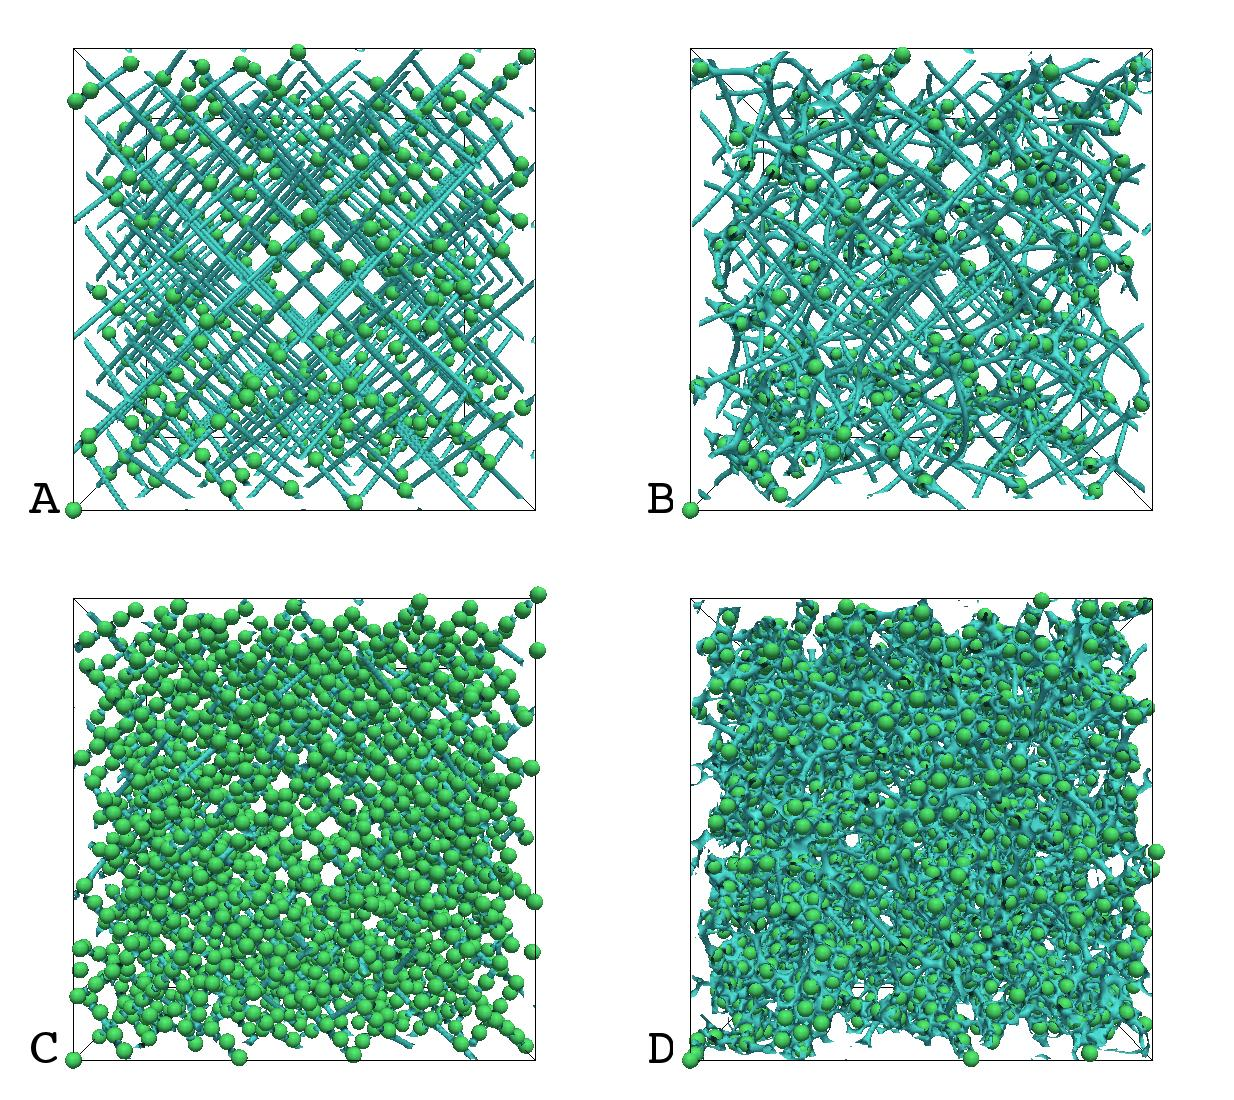
\includegraphics[scale=0.35]{s1.jpg}
\end{center}
\caption{As for main manuscript Fig.~1 (initialised to equilibrium blue
phase I), but for the entire simulation
system of 128$^3$ lattice sites. (a) solid volume fraction 1\% and
weak anchoring; (b) 1\% solid volume fraction and strong anchoring;
(c) 5\% solid volume fraction and weak anchoring; (d) 5\% solid
volume fraction and strong anchoring. The view direction in the
main figure is from the left here. There is a reference
particle at the bottom left in each panel which does not take part
in the simulation.}
\end{figure}

\begin{figure}
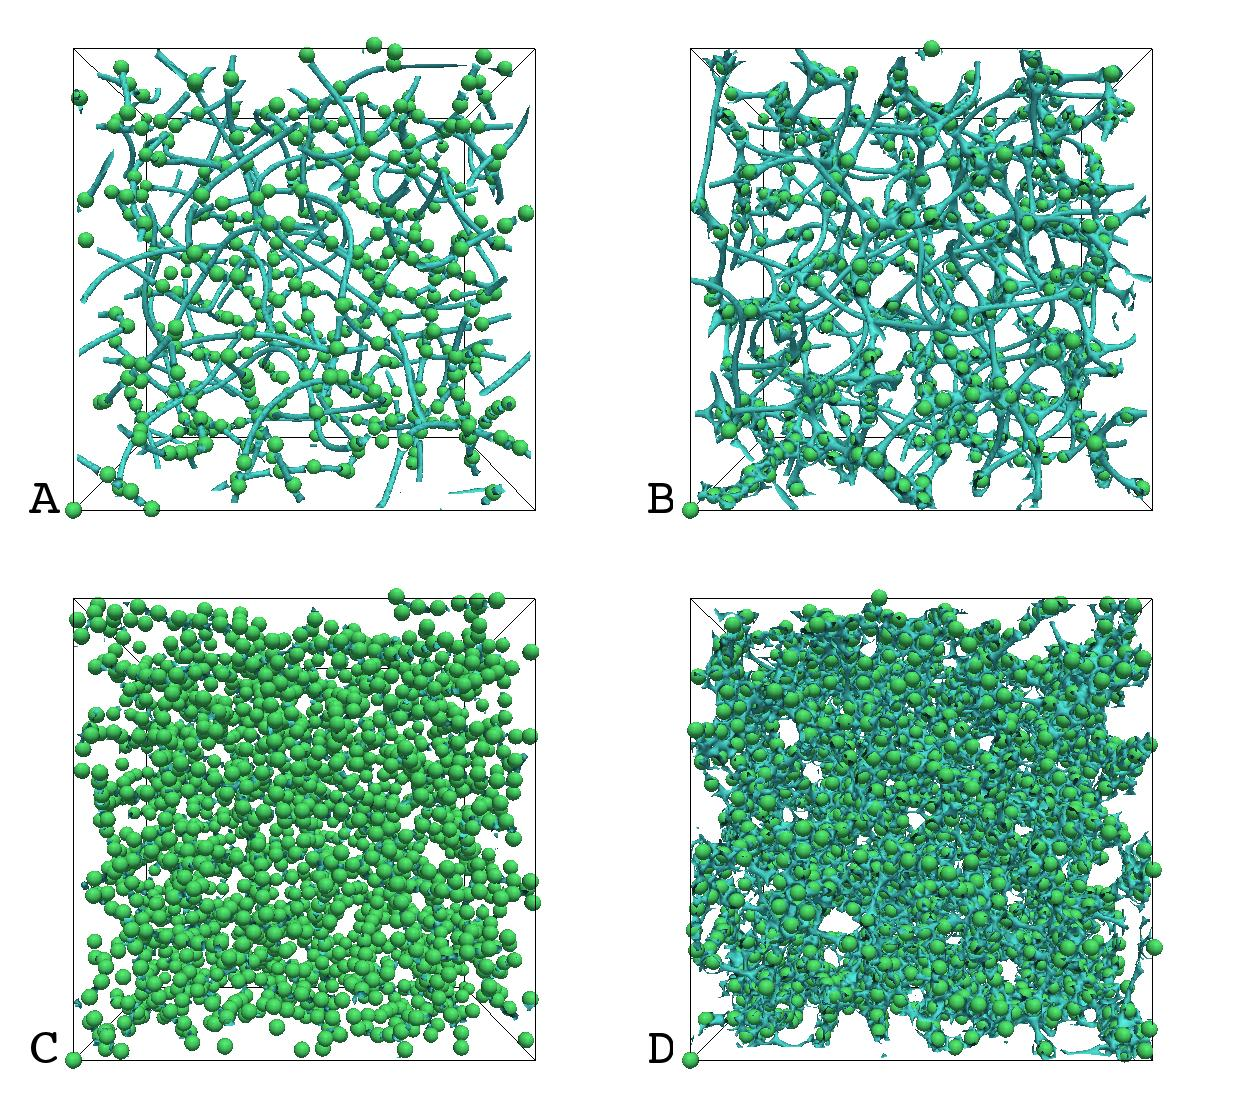
\includegraphics[scale=0.35]{s2.jpg}
\caption{As for main manuscript Fig.~2 (initialised via a ``quench''
to generate a disordered network), but for the entire simulation
system of 128$^3$ lattice sites. (a) solid volume fraction 1\% and
weak anchoring; (b) 1\% solid volume fraction and strong anchoring;
(c) 5\% solid volume fraction and weak anchoring; (d) 5\% solid
volume fraction and strong anchoring. Again, there is a reference
particle at the bottom left in each case which does not take part
in the simulation.}
\end{figure}

\begin{figure}
\begin{center}
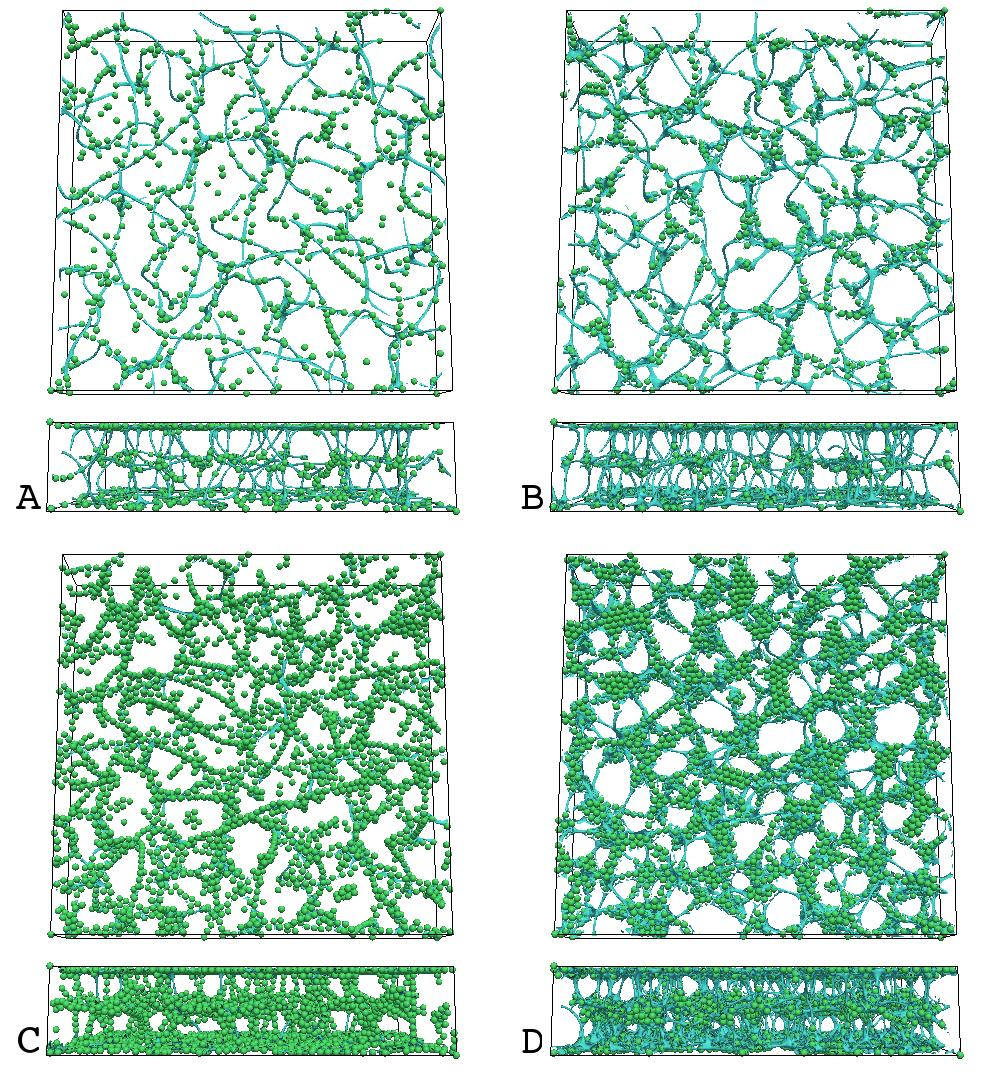
\includegraphics[scale=0.42]{s3.jpg}
\end{center}
\caption{As for main manuscript Fig.~3 (confined geometry with normal
anchoring walls at both top and bottom), but for the entire simulation
system of 256$^2\times$56 lattice sites. Each shows a top view and
side view of the same simulation state. (a) solid volume fraction 1\%
and weak anchoring; (b) 1\% solid volume fraction and strong anchoring;
(c) 4\% solid volume fraction and weak anchoring; (d) 4\% solid
volume fraction and strong anchoring.}
\end{figure}

\begin{figure}
\begin{center}
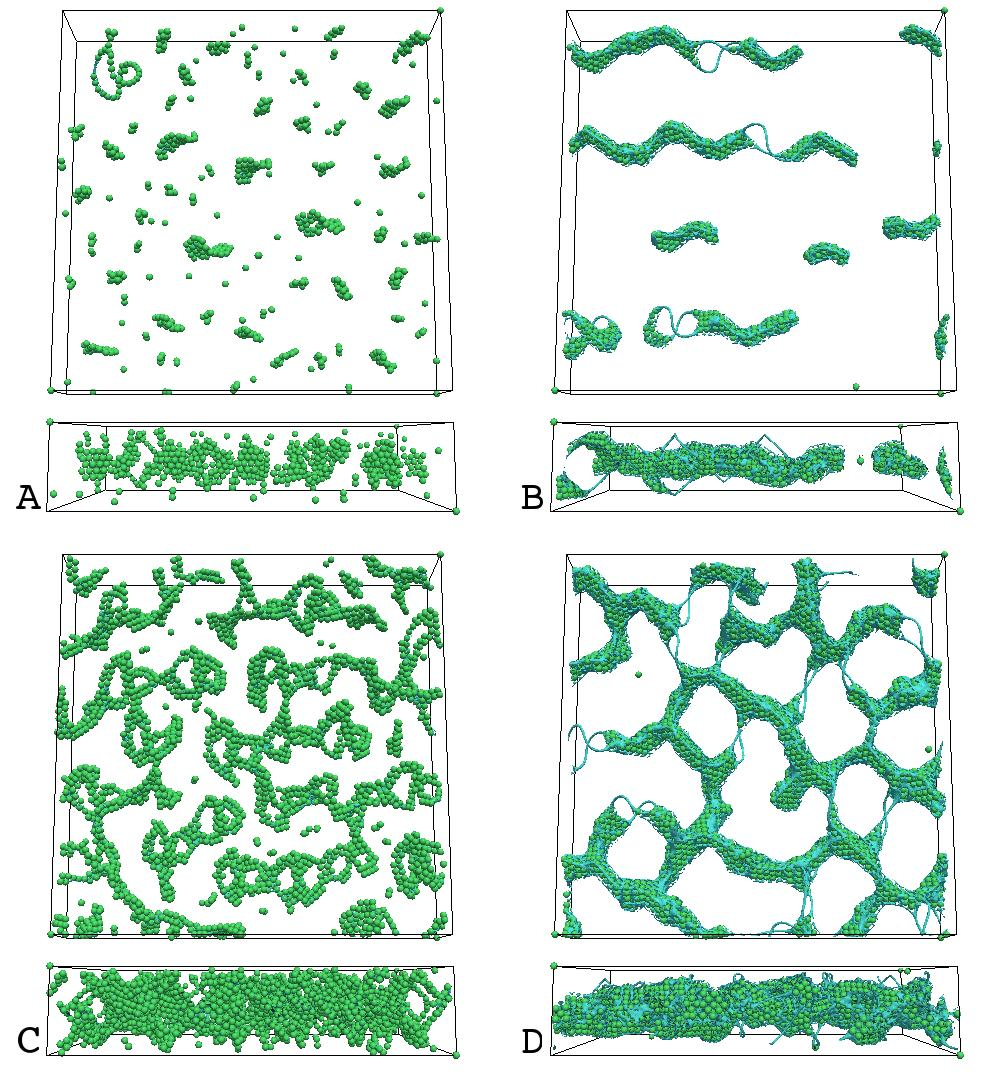
\includegraphics[scale=0.42]{s4.jpg}
\end{center}
\caption{As for main manuscript Fig.~4 (confined geometry with planar
anchoring walls at both top and bottom), but for the entire simulation
system of 256$^2\times$56 lattice sites. Each shows a top view and
side view of the same simulation state. (a) colloid solid volume fraction 1\%
and weak anchoring; (b) 1\% solid volume fraction and strong anchoring;
(c) 4\% solid volume fraction and weak anchoring; (d) 4\% solid
volume fraction and strong anchoring.}
\end{figure}

\begin{figure}
\begin{center}
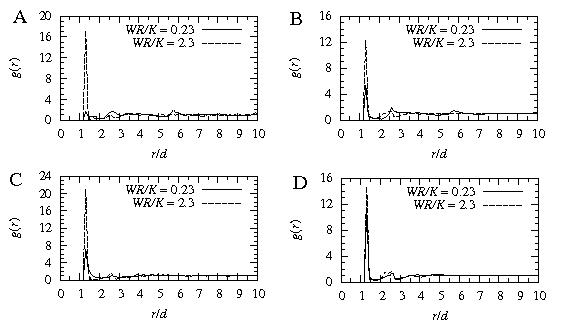
\includegraphics[width=0.95\columnwidth]{s5.jpg}
\end{center}
\caption{Pair correlation function for weak ($WR/K=0.23$) and strong ($WR/K=2.3$) anchoring cases considered in the manuscript. (A,B) BPI initialisation with A) volume fraction $\phi=1${\%} and B) $\phi=5${\%}. (C,D) ``quenched system'' with C) $\phi=1${\%} and D) $\phi=5${\%}.}
\end{figure}

\newpage

{\bf Supporting References}

\begin{thebibliography}{99}

\bibitem{blue1}
D.C. Wright and N.D. Mermin,
%  Crystalline liquids -- the blue phases.
{\it Rev. Mod. Phys.} {\bf 61,} 385-432 (1989).

%\bibitem{marendu1}
%D. Marenduzzo, E.  Orlandini, M. E. Cates, J. M. Yeomans,
%{\rm Steady-state hydrodynamic instabilities of active liquid crystals:
%Hybrid lattice Boltzmann simulations.}
%{\it Phys. Rev. E} {\bf 76}, 031921 (2007).

%\bibitem{marendu2}
%O. Henrich, D. Marenduzzo, K. Stratford, M. E. Cates, 
%{\rm Domain growth in cholesteric blue phases:
%hybrid lattice Boltzmann simulations}.
%{\it Comput. Math. Appl.}, doi:10.1016/j.camwa.2009.08.047[dx.doi.org] (2009).

%\bibitem{marendu3}
%M. E. Cates, O. Henrich, D. Marenduzzo, K. Stratford,
%{\rm  Lattice Boltzmann simulations of liquid crystalline fluids:
%active gels and blue phases.}
%{\it Soft Matter} {\bf 5}, 3791-3800 (2009).

\bibitem{oliver1}
O. Henrich, D. Marenduzzo, K. Stratford, and M.E. Cates,
%Thermodynamics of blue phases in electric fields
\textit{Phys. Rev. E}, \textbf{81} 031706 (2010).

\bibitem{beris}
A. N. Beris, B. J. Edwards, 
{\it Thermodynamics of Flowing Systems with Internal Microstructure}
(Oxford Univ. Press, New York, 1994).

\bibitem{deGennes}
P.-G. de Gennes, J. Prost,
{\it The Physics of Liquid Crystals} (Oxford Univ. Press, New York, 1993).

\bibitem{ladd94}
A.J.C. Ladd,
\textit{J. Fluid Mech.} \textbf{271}, 285 (1994); \textit{ibid.} \textbf{271}
311 (1994).

\bibitem{nguyen2002}
N.-Q. Nguyen and A.J.C. Ladd,
\textit{Phys. Rev. E} \textbf{66} 046708 (2002).

\bibitem{fournier2005}
J.-B. Fournier and P. Galatola,
\textit{Europhys. Lett.} \textbf{72}, 403 (2005).

\end{thebibliography}



\end{document}


% MY NOTES

KEVIN

All particle radius $a = 2.3$.

Fluid properties: $\rho_0 = 1$; $\eta = 0.01$; $\zeta = 10\eta$;
temperature $T =2.133333 10^{-9}$.

Free energy:
$A_0 = 0.01$; $\gamma = 3.085143$; $q_0 = 0.09817477$ (and $p = 64$);
$\kappa_1 = \kappa_2 = 0.018971857$;
Chirality $\bar{\kappa} = 0.8$; $\tau = -0.25$

Amplitude order $ 0.0001$; Computed surface order $0.3509236$;
Rotational diffusion $\Gamma = 0.5$
Initialisation is 'random'.

Wall surface $W = 0.018971957$, ie., $W/\kappa$ = 1 length

Weak colloid anchoring $W = 0.0018971957$, ie., $W/\kappa = 0.1$ length
and $Wa/\kappa = 0.23$.

Strong colloid anchoring $W = 0.037943914$, ie., $W/\kappa = 2.0$ length
or $Wa/\kappa = 4.6$.


JUHO (BPI)



Fluid properties: $\rho_0 = 1$; $\eta = 0.01$; $\zeta = \eta$;
Temperature: $T = 2.133333 10^{-9}$. 

Free energy: $A_0 = 0.01$; $\gamma = 3.0$; $q_0 = 0.13884$; (and $p = 45.25$
is $32\sqrt{2}$);
$\kappa_1 = \kappa_2 = 0.00706095$;
Chirality $\bar{\kappa} = 0.7$ Reduced temperature $\tau = 0.0$.

Amplitude of order $-0.2$; Computed surface order:
Rotational diffusion $\Gamma = 0.5$

Wall irrelevant

Weak colloid anchoring $W = 0.000706095$, ie., $W/\kappa = 0.1$ length
and $Wa / \kappa = 2.3$.

Strong colloid anchoring $W = 0.00706095$, i.e., $W/\kappa = 1.0$
and $Wa/\kappa = 1.0$.



JUHO (QUENCH)

Fluid properties: $\rho_0 = 1$; $\eta = 0.01$; $\zeta = \eta$;
Temperature: $T = 2.133333 10^{-9}$. 

Free energy: $A_0 = 0.01$; $\gamma = 3.1$; $q_0 = 0.13884$; (and $p = 45.25$
is $32\sqrt{2}$);
$\kappa_1 = \kappa_2 = 0.00706095$;
Chirality $\bar{\kappa} = 0.68862$ Reduced temperature $\tau = -2.90322$.
